%!TEX root = main.tex
%\ProvidesPackage{config}

%\RequirePackage{silence}
%\WarningFilter{biblatex}{Patching footnotes failed}
\documentclass[11pt]{beamer}
\usepackage[utf8]{inputenc}
\usepackage[T1]{fontenc}

\usepackage[frenchb]{babel}
\usepackage{todonotes}
\usepackage{color}
\usepackage{bm} % \bm{} for bold font in text and math modes
\usepackage{caption,subcaption} % subcaption -> \begin{subfigure}
\usepackage{relsize}
\usepackage{booktabs,tabularx}
\usepackage{pifont} % for using \ding{}


\definecolor{green2}{RGB}{0.0,0.5,0.0}
\newcommand{\cmark}{\textcolor[rgb]{0.0,0.5,0.0}{\ding{51}}}% "check" mark
\newcommand{\xmark}{\textcolor{red}{\ding{55}}}% "cross" mark
\usepackage{amsmath}
\usepackage{amssymb}
\usepackage{booktabs,tabularx}
\usepackage{tikz}
\usetikzlibrary{arrows.meta,shapes.arrows}

\usepackage[backend=biber,style=ieee-alphabetic,date=long,maxbibnames=5,language=english]{biblatex}
\renewcommand{\UrlFont}{\ttfamily}


\usetheme{Warsaw}
\usefonttheme[onlymath]{serif}
\setbeamertemplate{footline}{~\insertframenumber/\inserttotalframenumber~} % Display slide numbering "2/30"
\setbeamertemplate{navigation symbols}{}



\bibliography{master-thesis.bib}


\AtBeginSection
{
\begin{frame}
		\tableofcontents[currentsection, hideothersubsections]
\end{frame}
}

% To suppress the page numbering of References at the end
\newcommand{\backupbegin}{
   \newcounter{framenumberappendix}
   \setcounter{framenumberappendix}{\value{framenumber}}
}
\newcommand{\backupend}{
   \addtocounter{framenumberappendix}{-\value{framenumber}}
   \addtocounter{framenumber}{\value{framenumberappendix}} 
}

% Because \begin{center} adds huge whitespaces
\newenvironment{tightcenter}{%
  \setlength\topsep{0pt}
  \setlength\parskip{0pt}
  \begin{center}
}{%
  \end{center}
}
  % Les usepackage sont dans config.tex
%%%%%%%%%%%%%%%%%%%%%%%%%%%%%%%%%%%%%%%%%%%%%%%%%%%%%%%%%%%
% MACROS
%%%%%%%%%%%%%%%%%%%%%%%%%%%%%%%%%%%%%%%%%%%%%%%%%%%%%%%%%%%

% Couleurs pour les corrections
\newcommand {\JY}[1] {\textcolor{red}{#1}}
\newcommand {\FR}[1] {\textcolor[rgb]{0.0,0.3,0.0}{#1}}
\newcommand {\OL}[1] {\textcolor{blue}{#1}}
\newcommand {\HW}[1] {\textcolor[rgb]{0.3,0.2,0.0}{#1}}
%\newcommand{\hilite}[1] {\emph{#1}}
\newcommand{\hilite}[1] {\Req{#1}}
\newcommand {\Req}[1] {\textcolor[rgb]{0.75,0.0,0.0}{#1}}
\newcommand {\Geq}[1] {\textcolor[rgb]{0.0,0.5,0.0}{#1}}
\newcommand {\Beq}[1] {\textcolor[rgb]{0.0,0.15,0.60}{#1}}
\newcommand {\black}[1] {\textcolor{black}{#1}}

% Espaces mathématiques
\newcommand {\DPUN} {{\mathcal D}}
\newcommand {\DTREE} {{\mathcal D}^e}
\newcommand {\CC} {\mathbb C}
\newcommand {\RR} {\mathbb R}
\newcommand {\RP} {\mathbb R^{\mathcal P}}
\newcommand {\RPE} {\mathbb R^{\mathcal P \times |\edges |}}
\newcommand {\codeset} {\mathbb R^{\mathcal P \times \leaves}}
\newcommand {\Dset} {\mathbb R^{\mathcal P \times (\mathcal P \#\leaves) }}
\newcommand {\ZZ} {\mathbb Z}
\newcommand {\NN} {\mathbb N}
\newcommand {\PP} {{\mathcal P}}
\newcommand {\HH} {{\mathbb H}}
\newcommand {\II} {{\mathbb I}}
\renewcommand {\SS} {{\mathcal S}} % applis supports
\newcommand {\SA} {{\mathbb S}} % support accessible

% Fonctions
\newcommand {\f}[1] { {\mathcal F}\left( #1 \right) }
\newcommand {\F}[1] { {\mathcal F^{-1}}\left( #1 \right) }
\newcommand {\norm}[2] {\left\| #1 \right\| _{#2}}
\newcommand {\defeq} {\triangleq}

% Opérateurs
\DeclareMathOperator {\sign} {sign}
\DeclareMathOperator {\prox} {prox}
\DeclareMathOperator {\argmin} {argmin}
\DeclareMathOperator {\supp} {supp}
\DeclareMathOperator {\rg} {rg}
\DeclareMathOperator {\diag} {diag}
\newcommand {\RG}[1] {\rg\left( #1 \right)}
\newcommand {\SUPP}[1] {\supp\left( #1 \right)}
\newcommand {\PS}[2] {\langle #1 , #2 \rangle}
\newcommand {\PROBA}[1] {\mathbb P \left( #1 \right)}
\newcommand {\one}[1] {\mathbbm{1}_{ #1 }}
%\newcommand {\one}[1] {\chi_{ #1 }} %{\mathbbm{1}_{ #1 }}
\newcommand {\oneinf}[1] {\chi_{ #1 }}
%\newcommand {\oneinf}[1] {{\mathcal I}_{ #1 }} 

% Acronymes
\newcommand {\PSNR} { \textrm{PSNR}^* } 
\newcommand {\NRE} { \textrm{NRE} }
\newcommand {\CPR} { \textrm{RER} }
\newcommand {\COST} { \textrm{G} } % ancien compression ratio

% Raccourcis
\newtheorem{prop}{Proposition}[section]

\newcommand {\nodes} {\mathcal N}
\newcommand {\edges} {\mathcal E}
\newcommand {\leaves} {\mathcal F}
\newcommand {\NL} {\#\leaves}
\newcommand {\hall} {h^e _{e \in \edges}}
%\newcommand {\multiconv}[1] { \bigstar_{\substack{#1}}\, }
\newcommand {\multiconv}[1] { \mathbf h^{#1}\, }
\newcommand {\tpath}[1] {\mathcal{C}(#1)}
\newcommand {\code} {\mathbf x}
\newcommand {\data} {\mathbf y}
\newcommand {\dataex} {\mathbf b}
\newcommand {\databis} {\mathbf y^e}
\newcommand {\D} {\mathbf D}
\newcommand {\Hs} {\mathbf A}
\newcommand {\Ha} {\mathbf H}
\newcommand {\Haf} {\hat{\mathbf H}}
\newcommand {\Hab} {\bar{\mathbf H}}
\newcommand {\res} {\mathbf r}

\newcommand {\tree}{\mathcal T}
\newcommand{\subtree}[1]{\tree^{#1}}

\newcommand {\stopalgo}{\epsilon}

% autres MACROS
\newcommand {\hkall} {(h^k)_{1 \leq k \leq K}}
\newcommand {\hkconv} {h^1 * \dots * h^K}
\newcommand {\hkconvnorm} {\frac{h^1}{\norm{h^1}{2}} * \dots * \frac{h^K}{\norm{h^K}{2}}}
\newcommand {\hkconvp} {g^{1} * \dots * g{K}}
\newcommand {\hkconvs} {f^{1} * \dots * f^{K}}
\newcommand {\fobj} {\| \code * h^1 * \dots * h^K - \data \|_2^2}
\newcommand {\fobjlambda} {\| \lambda \code * h^1 * \dots * h^K - \data \|_2^2} % Présentation d'O. Chabiron



\title{Optimisation de dictionnaires structurés en arbres de convolutions pour la représentation parcimonieuse d'images}
\subtitle{Stage encadrée par\\François Malgouyres (IMT), Jean-Yves Tourneret (IRIT-ENSEEIHT) et Herwig Wendt (CNRS-ENSEEIHT)}

\date{Soutenance de stage du 8 septembre 2016}
\author{Maël Valais}
%\institute{}

\begin{document}

\maketitle

\plain{Introduction : \\la représentation parcimonieuse}


\begin{frame}[label=LO]{La représentation parcimonieuse}
La \alert{représentation parcimonieuse} permet de débruiter, décrire, compresser, classifier
\todo[inline]{TODO: ajouter exemple image débruitée avec KSVD}
\end{frame}


\begin{frame}{Les dictionnaires}
Dictionnaire = opérateur permettant de passer d'une image à une représentation cible

\end{frame}


\begin{frame}{Dictionnaires génériques vs. appris}
\begin{description}
	\item[Dictionnaires génériques] cosinus (JPEG), Fourier, Wavelets, Curvelets
	\item[Dictionnaires appris] K-SVD
\end{description}
\end{frame}


\begin{frame}{Problème du coût de Dx}
Problème d'apprentissage de dictionnaire \eqref{eq_dl} pour apprendre un dictionnaire parcimonieux :
\begin{align} 
\underset{\D,\x}{\min}~ & \| \x \|_1 + \lambda \| \Req{\D\x}-\y \|^2_2 \tag{$DL$}\label{eq_dl} \\
\text{s.t.}~ & \| \d_k \| \le \gamma & \forall k = 1,\dots,K\label{eq_dl_finite_norm} \notag
\end{align}
\begin{description}
	\item[Problème] Coût élevé de $\D\x$ : \alert{$O(N^2)$}
	\item[Solution] Réduire la taille des images en entrée (patches dans KSVD)
	\item[Défaut] Les atomes ne peuvent pas représenter de grandes formes
\end{description}
\end{frame}


\begin{frame}{Motivations générales}
	\begin{itemize}
		\item développer une \alert{transformée rapide} adaptée aux grands atomes
		\item effectuer l'apprentissage \alert{directement sur l'image} au lieu des patches
	\end{itemize}
\end{frame}


\plain{Existant : \\Modèle d'arbre convolutionnel et PALMTREE}

\begin{frame}{Existant : le modèle d'arbres de convolutions}
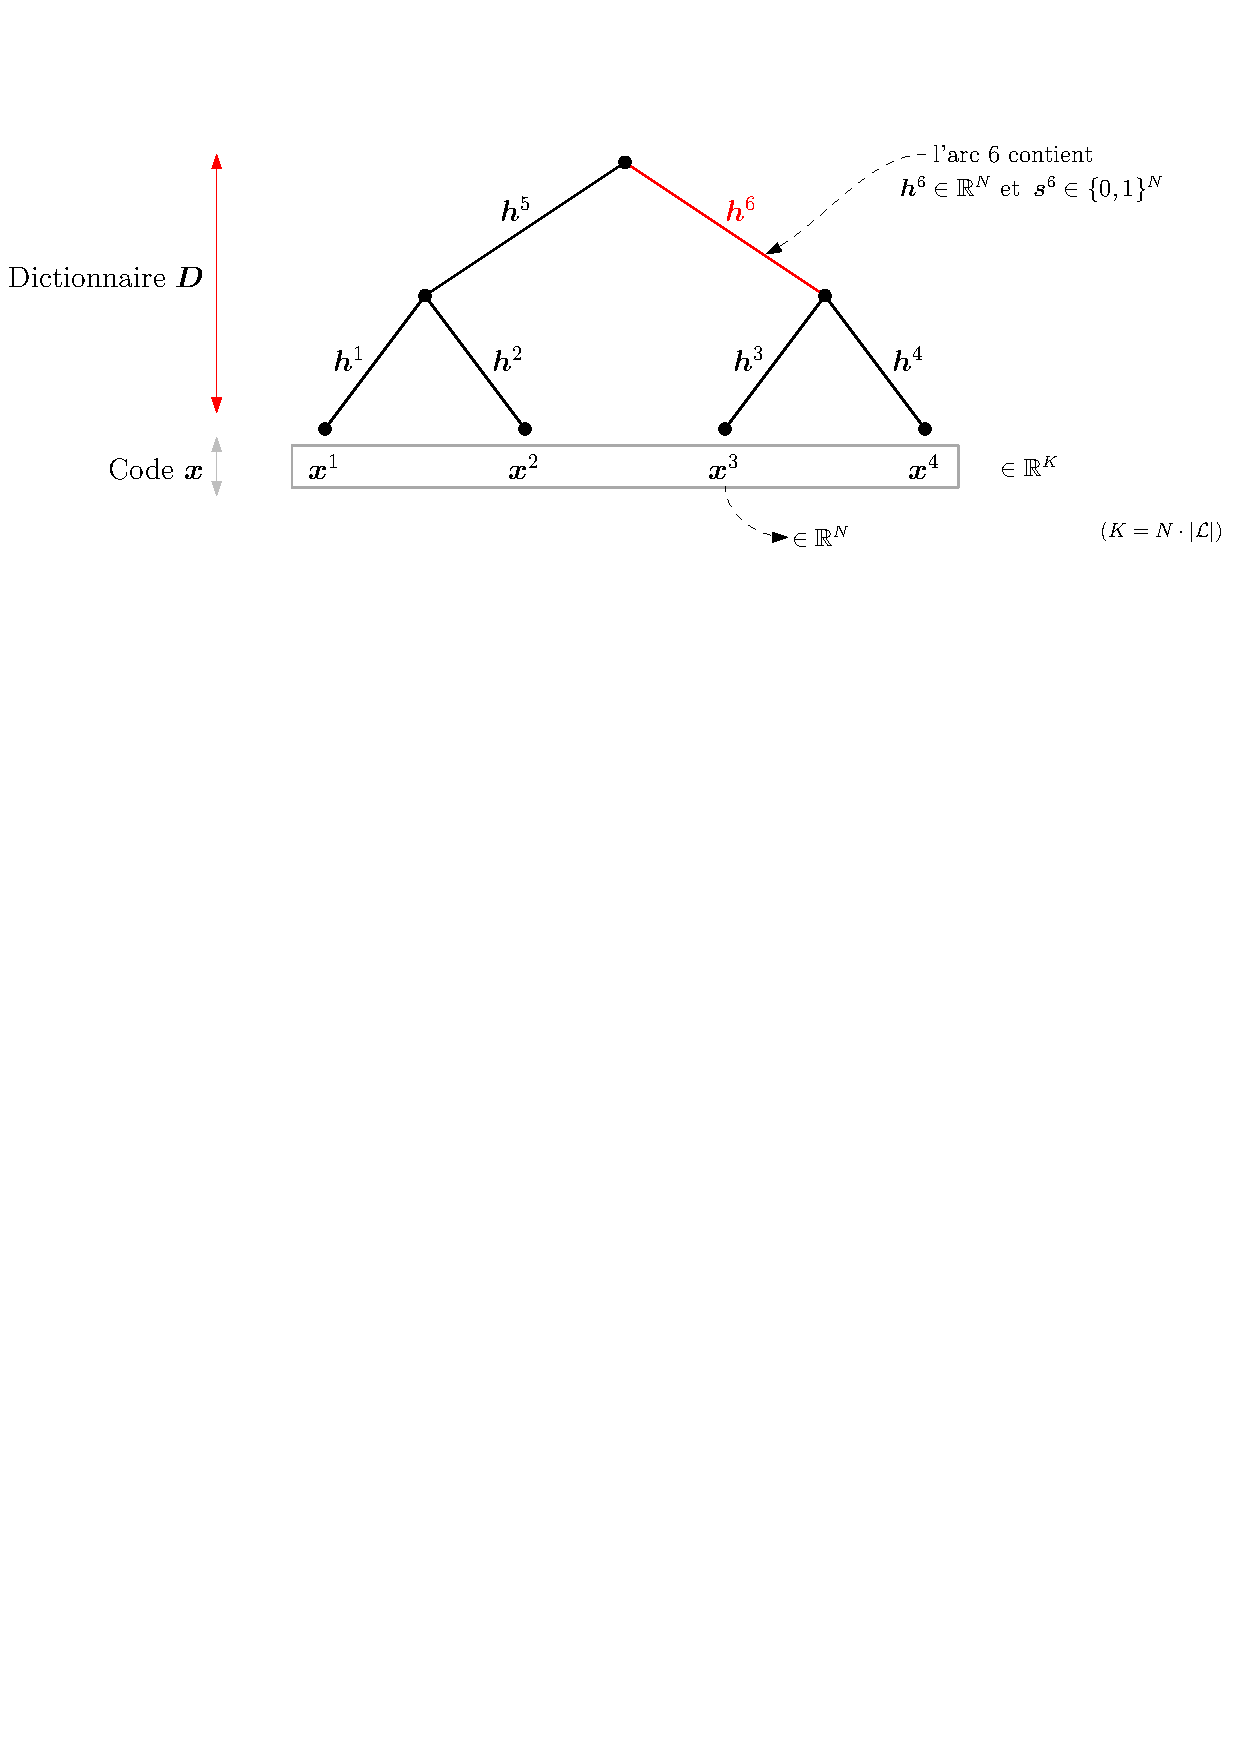
\includegraphics[width=\textwidth]{figures/tree.pdf}

Ainsi, le produit $\D\x$ est réduit à

\begin{equation}
\D \x = \Req{\sum_{l \in ~\text{Feuilles}}} \x^{\Req{l}} * \underbrace{\h^{\Req{l}}* \dots* \h^{r}}_{\textrm{de la racine à la feuille}}
\end{equation}
soit une complexité en \alert{$O(N)$}

\end{frame}


\begin{frame}{Existant : problème associé}
On appelle \eqref{eq_ftl} (\alert{Fast Transform Learning}) l'adaptation de \eqref{eq_dl} à ce modèle :
\begin{equation*} {\small
\underset{\substack{(\h^\text{e})_{e \in \E}}}\min
	\norm{\Req{\sum_{l \in Feuilles}} \x^{\Req{l}} * \h^{*\Req{l}} -\y}{2}^2 \tag{${FTL}$} \label{eq_ftl}
    }
\end{equation*}
L'algorithme \alert{PALMTREE} donne une solution à ce problème.
\end{frame}


\begin{frame}{Existant : algorithme PALMTREE}
	\todo[inline]{quelques mots sur les étapes de PALMTREE}
\end{frame}


\begin{frame}{Existant : résultats et défauts}
	\todo[inline]{image de 16 curvelet approchées}
\end{frame}

\begin{frame}
	\frametitle{Objectifs du stage}
	Étudier la possibilité d'apprendre les supports à partir de l'image cible
\end{frame}


\plain{Travail réalisé}

\begin{frame}{L'idée}
\begin{itemize}
	\item Apprendre le support "à la OMP"
	\item Utiliser la direction de plus forte descente du gradient
\end{itemize}
Dans les faits, il a fallu
\begin{itemize}
	\item Vérifier que le gradient indique bien le meilleur élément à ajouter au support
	\item Vérifier que l'algo OMP-PALMTREE fonctionne sur un arbre
\end{itemize}
\end{frame}


\begin{frame}{Ajouter un élément au support avec le gradient?}
\end{frame}


\begin{frame}{OMP-PALMTREE sur une branche}
\end{frame}


\begin{frame}{OMP-PALMTREE sur un arbre}
Soucis
\begin{itemize}
	\item les éléments de chaque supports sont très éloignés les uns des autres
	\item la taille du support est déséquilibrée à travers l'arbre
\end{itemize}
\end{frame}


\begin{frame}{Régularisation}
\end{frame}


\begin{frame}{En quelques mots...}
\begin{itemize}
\item PALMTREE (existant) se base sur des arbres de convolutions
\item Passer des supports fixes (PALMTREE) à des supports appris (OMP-PALMTREE)
\item ...
\end{itemize}
\vfill
\hfill Merci de votre attention
\end{frame}

\appendix

\begin{frame}[allowframebreaks,noframenumbering]
\frametitle{Bibliographie de l'équipe}
\nocite{*}
\printbibliography[heading=none]
\end{frame}


\end{document}